\section{Corpus Construction and Provenance}
\label{app:corpus}

\emph{Four} public sources are pooled onto a shared legacy block vocabulary
(the text2mc dump is remapped with $97\%$ block-state coverage; world cuts are
ground-stripped), passed through a quality gate, and deduplicated variant-aware.
The fourth source, \texttt{text2mc\_schem}, is the set of raw \texttt{.schem}
files in the text2mc release that its authors never converted. It entered the
pool after the $32^3$ cache was built, so that cache draws on three sources and
only the $48^3$ cache carries all four. The main text (\S\ref{sec:setting}) describes the three that build
\texttt{houses\_32}, the corpus every reported run uses.

\begin{table}[h]
\centering
\small
\caption{Corpus construction, transcribed from the cache manifests. Per-source
columns are post-gate, post-deduplication counts and sum to \textbf{final};
\textbf{final} is \emph{pooled} less \emph{drops} less \emph{dups}. Material
variants, the same shape in different materials, are \emph{kept} and not
deduplicated.}
\setlength{\tabcolsep}{4pt}
\begin{tabular}{lrrrrrrrr}
\toprule
      &        & quality & exact  &                  &           &          &         & text2mc \\
cache & pooled & drops   & dups   & \textbf{final} & GrabCraft & 3D-Craft & text2mc & \texttt{\_schem} \\
\midrule
\texttt{houses\_32} & 3{,}493 & 826 & 6 & \textbf{2{,}661} & 1{,}360 & 1{,}267 & 34 & --- \\
\texttt{houses\_48} & 4{,}502 & 1{,}381 & 33 & \textbf{3{,}088} & 1{,}410 & 1{,}381 & 180 & 117 \\
\bottomrule
\end{tabular}
\end{table}

Drop reasons at $32^3$, $826$ in total: no interior $675$, single-material blob
$52$, fragmented $37$, too flat $29$, fewer than three materials $22$, too
sparse $9$, too few blocks $2$.

\paragraph{The enclosed-air gate is calibrated per source.}
The gate requires at least $8$ interior air voxels unreachable from the bounding
box boundary. Measured on ground truth, $17\%$ of GrabCraft houses legitimately
have open interiors, against $31\%$ of 3D-Craft and $54\%$ of text2mc, so
GrabCraft is exempted from the gate and the other three are not.
\texttt{text2mc\_schem} is gated on the same grounds as the rest of the text2mc
release and is not calibrated separately. What the gate removes from the gated
sources is trees, a truck and roof fragments, read off a pre-gate visual grid.

\section{Descriptor Ablation}
\label{app:descriptor}

Two objections apply to any handcrafted descriptor. The first is that \vkid{}
separates \solidify{} only because the probe adds mass, and the descriptor
contains an explicit size term. The second is that it separates \solidify{} only
because the descriptor contains a sealed-interior scalar that the probe drives to
zero. We test both by deleting the terms and by matching the mass.

Table~\ref{tab:descriptor-ablation} reports every variant at $n{=}128$ with $48$
fresh real draws per variant, each in its own noise floor, so a column compares
variants and not raw distances. Deleting the size term \texttt{log1p\_n\_blocks}
moves the separation from $201.8$ to $202.2$. Deleting
\texttt{interior\_ratio\_sealed} moves it to $197.1$. Deleting both leaves
$197.3$. Neither term carries the result. No single block reproduces it alone
either: the strongest, the nine global scalars, reaches $164.5$ on $9$
dimensions, and the $55$ pattern bins that dominate the descriptor by dimension
reach $113.9$.

\growshell{} settles the mass question directly. It dilates the solid outward
until it has added exactly the number of blocks \solidify{} adds to that build,
which it achieves to within one block on $128$ of $128$ builds at a median of
$196$ added blocks. Same builds, same material, same mass, and the only
difference is whether the new mass lands inside or outside. The two tiers then
separate completely: \mvkid{} reads $+0.26$ noise floors on \solidify{} and
$+102.27$ on \growshell{}, while \vkid{} reads $201.8$ and $214.5$. A descriptor
that counted blocks could not produce that pair of rows.

\begin{table}[!htb]
\centering
\small
\caption{Descriptor ablation, $n{=}128$, $48$ real draws per variant. Each
separation is in that variant's own noise floor, measured under that variant.
The two suspect terms are the explicit size scalar and the sealed-interior
scalar; deleting either or both leaves the separation intact.}
\label{tab:descriptor-ablation}
\setlength{\tabcolsep}{5pt}
\begin{tabular}{lrrrr}
\toprule
descriptor variant & dims & floor & \solidify{} & \growshell{} \\
\midrule
full                              & $77$ & $0.1097$ & $\mathbf{201.8}$ & $214.5$ \\
\midrule
\multicolumn{5}{l}{\emph{deleting a suspect term}} \\
without \texttt{log1p\_n\_blocks}       & $76$ & $0.1114$ & $202.2$ & $214.9$ \\
without \texttt{interior\_ratio\_sealed}& $76$ & $0.1127$ & $197.1$ & $211.7$ \\
without both                            & $75$ & $0.1147$ & $197.3$ & $211.9$ \\
\midrule
\multicolumn{5}{l}{\emph{deleting a whole block}} \\
without pattern bins    & $22$ & $0.5113$ & $198.0$ & $120.9$ \\
without wall thickness  & $72$ & $0.1163$ & $176.4$ & $216.6$ \\
without height profile  & $69$ & $0.1312$ & $199.6$ & $213.9$ \\
without global scalars  & $68$ & $0.1302$ & $171.6$ & $206.7$ \\
\midrule
\multicolumn{5}{l}{\emph{one block alone}} \\
pattern bins only       & $55$ & $0.1802$ & $113.9$ & $201.3$ \\
wall thickness only     & $5$  & $6.0167$ & $158.7$ & $75.7$ \\
height profile only     & $8$  & $1.6293$ & $8.0$   & $28.9$ \\
global scalars only     & $9$  & $1.7594$ & $164.5$ & $118.1$ \\
\bottomrule
\end{tabular}
\end{table}


\section{Reproducibility}
\label{app:repro}

\TODO{Fill in at submission: anonymized code URL, exact commit, the pinned split
files, the feature-cache render canary hash, hardware, and per-run wall-clock.
The suite writes a scorecard carrying corpus, split, $n$, reference size, seed,
host, device and git SHA for every run, so this table is a transcription rather
than a reconstruction.}

Two properties of the protocol matter for reproducibility:

\begin{itemize}[leftmargin=*,itemsep=1pt,topsep=2pt]
\item \textbf{Controls are re-scored in every run, never cached across runs.}
  \blockscore{}'s unit is the spread of the real control \emph{scored in the
  same run}, so two scores sit on one scale only when corpus, split, tier, seed,
  reference size and control size all match. We pin these as a named protocol
  and refuse to rank runs that do not satisfy it, listing each excluded run with
  its reason. The size of the control alone moves the score: the same model on
  the same corpus, split and tier scores $87.14$ against a $128$-build control
  and $19.05$ against a $32$-build one. A board that ignored the control's size
  would read that as a $4.5\times$ improvement.
\item \textbf{The calibration draw must be shuffled.} Taking the first $n$ test
  builds as the real-vs-real draw, rather than a shuffled sample, inflates the
  measured noise floor by $\mathbf{10.4\times}$ (s.d.\ $0.0318$ against $0.0030$
  at $n{=}128$) and shifts its center from $+0.0001$ to $+0.0404$. A contiguous
  block of a corpus stored in source and family order is not an exchangeable
  sample of it, so the floor it produces is both wider and displaced, and every
  separation measured against it is understated.
\item \textbf{Every arm must declare its training split} to be ranked, and an
  arm that cannot is reported unranked with that as the stated reason. No arm in
  the run reported here declares one (\S\ref{sec:casestudy:llm}). The
  requirement post-dates that run, so it is the fix rather than a gate that
  fired.
\end{itemize}

\paragraph{The language-model arms' decoding cap.} \llmft{} and \llmgeo{} decode at
temperature $0.8$ under a $1{,}200$-token cap. That cap is a real limitation of both arms:
$11$ of $128$ generations came back empty, $139$ attempts were needed for $128$ samples,
and several completions are truncated into structures one block thick
(Figure~\ref{fig:samples}). Raising the cap requires re-running the prompts, which we did
not do for this submission.

\section{Negative Results}
\label{app:negative}

Three experiments that did not work. Each bounds a claim a reader might
otherwise expect us to make about injecting structure into sequence models.

\paragraph{Attention is not a free adjacency prior.} A pretrained code LLM's
self-attention over a serialized build recovers less adjacency information than
the coordinates already printed in the prompt. Scoring all $336$ heads by how
well they rank the truly $6$-adjacent previous pieces (AUC over the causal
candidate set), the best head reaches $0.874$ in the base model and $0.884$
after task fine-tuning, well above a recency floor. But $-\|a_i - a_j\|_1$,
three lines of arithmetic over the coordinates the serialization already prints
on every line, scores $0.980$. A trained bilinear probe does better, $0.914$ at
layer $14$ of $28$, and falls to $0.807$ by the final layer, which is the layer
generation actually reads. There is signal; there is nothing to steal.

\paragraph{A shared relative-{3D} attention bias is a null, for a reason in the
parameterization.} Adding a learned additive attention bias indexed by the
relative {3D} offset between pieces, zero-initialized and otherwise holding the
fine-tune fixed, moved best validation loss by $-0.0021$ at one seed and did not
touch the collapse mode. The learned table explains why: $364$ of $729$ offset
buckets are \emph{never updated}. Under raster emission order every earlier
piece is sign-constrained, so half the offset space is unreachable by
construction, and the arm's entire learned signal is a reparameterization of
recency. Unlocking the rest requires a non-monotonic emission order. The
reference anchor is not the constraint: the dead half of the offset space
follows from monotonic emission alone.

\section{Counting Interiors}
\label{app:interior}

A naive enclosed-air count, restricted to air cells not reachable from the
bounding-box boundary, counts a room with an open doorway as no room at all. We
additionally close
the solid under a $26$-connected morphological closing that seals openings up to
two blocks wide and report the air that becomes enclosed only then. Calibrated
on a synthetic hollow cube with a $343$-cell room: a $1{\times}1$, $1{\times}2$
or $2{\times}2$ doorway recovers all $343$ cells; a $3{\times}3$ hole or a
missing wall recovers $0$, correctly classifying an open structure as having no
room. On the same $200$ held-out houses the probe statistics of
\S\ref{sec:probes} are measured on, $\mathbf{6.0\%}$ have no \emph{sealed}
interior at all, and \emph{every one} of those twelve builds does have a room
reachable through a doorway. Pooled over builds, apertures account for
$\mathbf{25.6\%}$ of total real interior volume, which is the margin by which a
sealed-only counter understates real houses. Every claim in the earlier literature,
and in our own prior notes, that generated builds ``have no interiors'' was made
with that counter.

\paragraph{The bootstrap $p$-value floor.}
A bootstrap sign-balance $p$-value is floored at $1/n_{\text{rep}}$, and Holm
over the $55$ pairs of an $11$-arm run multiplies $0.005$ to $0.275$. Nothing
can then reach $\alpha=0.05$ however large the true difference, which put
\emph{every} arm of an earlier head-to-head, from held-out real to a monochrome
corpus, in one ``not separated'' group. The reported $p$ is now studentized and
unfloored. The failure mode is silent: it produces a table in which nothing is
significant, which reads like a careful result.

The dose axis is calibrated by construction. \textsc{Partial-Fill} fills
interior cells \emph{inward from the walls}, nearest-first, which gives an
exactly calibrated dose (interior ratio $0.1175 \to 0.0941 \to 0.0708 \to
0.0475 \to 0.0242$). Two earlier designs were rejected. Random interior speckle
is detected as \emph{noise} rather than as lost interior. Filling whole rooms
largest-first makes the axis useless, because one dominant pocket is typically
more than a quarter of the total interior, so a nominal $25\%$ dose already
removes $71\%$ of it.

\section{Defects Found in Our Own Gates}
\label{app:defects}

These are the class of error a validation ladder exists to prevent, and it did
not.

\paragraph{Two defects in our own gates.} First,
$\mathrm{sd}(\text{real})$, the unit every gate is stated in, was mismeasured
twice. It was estimated from repeated subsamples of a pool that \emph{excluded}
the probe set, so the fresh real draw being tested was not a member of its own
null. Overlapping draws also carry a finite-population factor that shrinks their
spread. Corrected, a metric that separates the solidify probe at $67$ s.d.\ passes
the gate it had failed, having been rejected for noise that was measured wrong.
Second, the $n$-stability gate tested a difference of means against the spread
of a \emph{single} draw, larger by $\sqrt{\text{reps}}$, and therefore had almost
no power. Against the standard error of the difference, the biased estimator's
$1/n$ decay is rejected at $14.8$ standard errors.

\paragraph{A third defect, in the renderer.} A feature extractor that fails
open produces numbers that look excellent and cannot be caught downstream. Ours
substituted a blank white frame for any rendering exception. Under a library
version mismatch every render raised, every image came back white, every feature
collapsed to one vector, and every arm scored KID $=-4\times 10^{-13}$, better
than real. The feature cache is validated by a render canary, so the all-white
canary would have mismatched and the cache would have been silently rebuilt from
blank frames. The renderer now raises past a $2\%$ failure rate. Repairing the
library reproduced the stored canary hash bit-for-bit, so no previously recorded
number is affected.

\section{Full Tables}
\label{app:tables}

Tables reproduced here in full, including the results the main text reports only in
prose.

\begin{table}[t]
\centering
\small
\caption{Realism at $n{=}128$ against $399$ held-out real builds, with
bootstrap $95\%$ intervals. \textbf{\solidify{} is indistinguishable from
held-out real on the render metric} and $202$ spreads away on the geometric one.
The bottom two rows are the converse blindness: \vkid{} reads occupancy only,
so a material permutation moves it by \emph{exactly} zero (values are
bit-identical to the real row, not merely close).}
\label{tab:blindness}
\begin{tabular}{lcc}
\toprule
arm & \mvkid{} $\downarrow$ & \vkid{} $\downarrow$ \\
\midrule
\realheld{} (floor)       & $-0.001$ $[-0.004, 0.003]$ & $-0.09$ $[-0.22, 0.04]$ \\
\textbf{\solidify{}}   & $\mathbf{0.000}$ $[-0.002, 0.004]$ & $\mathbf{22.03}$ $[20.65, 23.70]$ \\
\matshuffle{}& $0.674$ $[0.644, 0.712]$ & \emph{$-0.09$ (bit-identical)} \\
\monochrome{}          & $0.930$ $[0.903, 0.962]$ & \emph{$-0.09$ (bit-identical)} \\
\traincopy{}          & $0.015$ $[0.007, 0.024]$ & $0.96$ $[0.60, 1.51]$ \\
\bottomrule
\end{tabular}
\end{table}

Table~\ref{tab:blindness} is the result. The solidified corpus reads $0.000$
against a real floor of $-0.001$.

\paragraph{Significance, not interval overlap.}
Marginal confidence intervals are not a comparison, because non-overlap demands
a difference roughly $41\%$ larger than significance does. We therefore test every
arm pair with the reference draw shared and apply Holm correction
\citep{holm1979simple} across the family. Under that test
\solidify{} and \realheld{} \textbf{share a significance
group} on \mvkid{}. The same test at the same $n$ assigns
\traincopy{} its own group at a difference of $0.015$, a separation that sits on the $\alpha{=}0.05$ boundary after Holm once the test is correctly calibrated (Appendix~\ref{app:significance}), which is why the main text argues the point by magnitude instead. On \vkid{}
the same solidified arm is four groups away, $\Delta = -22.13$
$[-24.08, -20.72]$, $p \approx 0$.


\subsection{Dose--Response}

Table~\ref{tab:dose} gives every rung of the dose-response sweep, and
Figure~\ref{fig:dose} plots the three axes. Table~\ref{tab:casestudy} gives the
head-to-head letters for the case-study arms, and Figure~\ref{fig:casestudy}
plots them with bootstrap intervals.

\begin{table}[t]
\centering
\small
\caption{Dose-response, $n{=}64$ per rung. \textbf{range (sd)} is the
best-to-worst span in units of the metric's own noise floor, given as
$n{=}64$\,/\,$n{=}128$ where both were run. The render metric is perfectly
monotone on two axes and \emph{flat} on the third; on that axis its rank
correlation is unstable between the two runs ($+0.300$ vs $+0.900$), being the
correlation of a sequence that does not move, so read the span instead. A
resolution axis was dropped: changing a build's resolution changes its size, not
its quality (\S\ref{sec:setting}).}
\label{tab:dose}
\begin{tabular}{llrcr}
\toprule
axis & metric & Spearman & monotone & range (sd) \\
\midrule
\multirow{2}{*}{\textbf{solidify} (interiors filled, $0\!\to\!100\%$)}
  & \vkid{} & $+1.000$ & yes & $\mathbf{133}$\,/\,$\mathbf{287}$ \\
  & \mvkid{}   & $+0.300$\,/\,$+0.900$ & \textbf{no} & $\mathbf{0.4}$\,/\,$\mathbf{1.1}$ \\
\midrule
\multirow{2}{*}{occupancy noise ($0\!\to\!20\%$ blocks moved)}
  & \vkid{} & $+1.000$ & yes & $226$ \\
  & \mvkid{}   & $+1.000$ & yes & $143$ \\
\midrule
\multirow{2}{*}{\textbf{mixture} (fraction of arm that is real)}
  & \vkid{} & $+1.000$ & yes & $105$ \\
  & \mvkid{}   & $+1.000$ & yes & $121$ \\
\bottomrule
\end{tabular}
\end{table}


\begin{table}[t]
\centering
\small
\caption{Retraining on a clean split collapses the margin. \vkid{} at
$n{=}128$, $399$-build reference, paired and Holm-corrected over all $153$ pairs
with an exact label-permutation test. Letters mark maximal sets of arms that no
test separated at $\alpha=0.05$: a shared letter means the pair was \emph{not
separated}, never that the arms are equivalent, and an arm carries several
letters when non-separation fails to be transitive, as it does here. The
contaminated arm is not separated from either its own clean retrain or the
stronger language-model baseline, and the clean retrain ties with both baselines
it had appeared to beat.}
\label{tab:casestudy}
\begin{tabular}{llrcl}
\toprule
& arm & \vkid{} $\downarrow$ & group & status \\
\midrule
& \realheld{} (floor)      & $-0.095$ & a & --- \\
& \traincopy{}         & $0.960$  & b & DQ memorization \\
\midrule
\multirow{4}{*}{\rotatebox{90}{\footnotesize submissions}}
& \voxar{}$^{\dagger}$ \emph{(contaminated)} & $11.624$ & \textbf{d} & unranked \\
& \textbf{\voxar{}} \emph{(clean)} & $14.898$ & \textbf{def} & ranked \\
& \llmft{}            & $15.006$ & \textbf{de} & ranked \\
& \llmgeo{}               & $15.869$ & \textbf{e} & ranked \\
& \voxarun{} \emph{(clean)} & $19.570$ & fgh & \textbf{DQ memorization} \\
\midrule
& \patchstitch{}               & $19.976$ & f & ranked \\
& \randomvox{}         & $37.729$ & j & ranked \\
\bottomrule
\end{tabular}
\end{table}


\begin{table}[t]
\centering
\small
\caption{Every arm, with its full recipe. The compact version is
Table~\ref{tab:arms} in \S\ref{sec:setting}.}
\label{tab:arms-full}
\begin{tabular}{llp{7.4cm}}
\toprule
kind & name & what it is \\
\midrule
floor      & \realheld{}      & held-out real builds from the test split, disjoint from the reference they are scored against \\
\midrule
probe      & \solidify{}      & every enclosed air cell filled with the build's own dominant material \\
probe      & \matshuffle{}    & the block multiset permuted across the build's own occupied cells: geometry exactly preserved \\
probe      & \monochrome{}    & every block replaced by one material: palette destroyed, geometry exactly preserved \\
probe      & \traincopy{}     & verbatim copies of training builds \\
probe      & \singlemode{}    & one build repeated $n$ times \\
\midrule
baseline   & \randomvox{}     & random voxels at the real occupancy density \\
baseline   & \hollowbox{}     & a hollow box: floor, walls, flat roof \\
baseline   & \gabled{}        & box, pitched roof, door, windows: a competent afternoon of rules \\
baseline   & \patchstitch{}   & $8^3$ patches lifted verbatim from \emph{different} real builds \\
baseline   & \copynoise{}     & a training build with $10\%$ of its blocks displaced \\
\midrule
submission & \voxar{}         & autoregressive transformer over merged-piece tokens, trained on the canonical split \\
submission & \voxarun{}       & the same model without orientation augmentation \\
submission & \llmft{}         & a fine-tuned code language model emitting one line per piece \\
submission & \llmgeo{}        & \llmft{} with a learned relative-{3D} attention bias \\
\bottomrule
\end{tabular}
\end{table}

Every control is re-scored in every run rather than cached, because a distance
means nothing until a floor has been measured under \emph{this} run's corpus,
split, $n$ and reference size. Importing a floor across runs ranks arms against
conditions they were never measured under.

\paragraph{What is not a control.} Earlier versions of this suite
included real data requantized to a coarser grid as a ranked control. We have
removed it. Decimation changes a structure's \emph{resolution}, not its
\emph{quality}, yielding a smaller building rather than a worse one, so a
leaderboard row for it invites the comparison ``this model is worse than
$86\%$-deleted real data,'' which is not a meaningful statement about quality.
It is removed from the validation ladder for the same reason and not merely from
the leaderboard: a ladder rung asks whether a metric orders a \emph{severity}
axis correctly, and decimation is not one, so a metric that ranks it any
particular way has demonstrated nothing. No result in this paper rests on a
decimation rung.

\subsection{Metrics}
\label{sec:metrics}

We use two realism metrics throughout, both the unbiased kernel two-sample
statistic of \citet{binkowski2018kid} and differing only in the features they
are computed on.

\begin{itemize}[leftmargin=*,itemsep=1pt,topsep=2pt]
\item \textbf{\mvkid{}}, the \emph{multi-view kernel distance}. Each structure is
  rendered from four orthographic views at $224$px and embedded with DINOv2-B
  \citep{oquab2024dinov2}. This is the render-and-embed family the field uses,
  and is our stand-in for it.
\item \textbf{\vkid{}}, the \emph{voxel kernel distance}. The same estimator on a
  $77$-dimensional descriptor computed directly on the voxel grid, with no
  rendering and no GPU. The dimensions are four blocks: the distribution over
  the $\mathbf{55}$ D4-orbits of $2\times2\times2$ occupancy patterns
  ($256$ patterns fall into $55$ orbits by Burnside's lemma under the order-$8$
  group of yaw rotations and an $x$-mirror), a $\mathbf{5}$-bin wall-thickness
  histogram, an $\mathbf{8}$-bin height profile normalized by the build's own
  height, and $\mathbf{9}$ global scalars. The group is exactly D4: a vertical
  flip is deliberately \emph{not} quotiented out, since upside-down is a real
  defect in a building, and we confirm it moves $45$ of the $77$ dimensions.
  Patterns are counted over the volume padded by one air cell, so surface
  patterns are counted rather than clipped at the border. The all-empty orbit is
  identically zero after normalization, leaving $76$ informative dimensions and,
  since each of the three histograms sums to one, $73$ free parameters.
\end{itemize}

\paragraph{Whitening and clipping.} Descriptor blocks differ by orders of
magnitude in scale, so the feature map whitens against statistics frozen on the
reference, \textbf{clips at $\pm 5$ reference standard deviations}, and then
L2-normalizes each row. The clip is load-bearing rather than cosmetic and we
report it for that reason: real houses have almost no mass five voxels deep, so
the reference standard deviation of the $\text{thickness} \geq 5$ bin is
$1.6\times10^{-4}$, and \solidify{} moves that single bin by $67.5$ reference
standard deviations before clipping. Without the clip one coordinate would
dominate the kernel, and the separation we report would be a one-dimensional
thickness test wearing a $77$-dimensional coat.

Both are reported in \emph{noise floors}: the spread of repeated real-vs-reference
draws at the same $n$. A value of $1$ means one sampling-noise unit away from
real, which makes the two commensurable despite differing by three orders of
magnitude in raw units.

\subsection{Metric Validation}

Table~\ref{tab:baselines} reports the procedural baselines against real held-out data,
Figure~\ref{fig:seven} plots Table~\ref{tab:seven}, Figure~\ref{fig:gallery} shows both
probe directions on three builds,
Figure~\ref{fig:pillars} plots the two pillars against each other, and
Figure~\ref{fig:descriptor} walks through the geometric descriptor.

Every candidate metric is scored on rungs of known damage, in units of its own
noise floor (the spread of real-vs-reference draws at the same $n$). Validity
gates are \emph{blocking}: a metric that fails one is reported as \emph{gated}
with the failing gate named, and may not appear in any ranking. Sensitivity, how
\emph{much} damage a metric resolves, is recorded separately, because
that is a question about $n$, not about whether the metric measures the right
thing.

\begin{table}[t]
\centering
\small
\caption{The render tier's metric-validation ladder (DINOv2-B, $4$ orthographic
views at $224$px, $n{=}64$). Columns are the probe rungs: real held-out, retype
$10\%$ of blocks (the rung the ordering gate uses for this tier), displace
$10\%$, delete $40\%$, material shuffle and a $90^\circ$ rotation; \textbf{sd}
is the metric's own noise floor. Gates are blocking, and \emph{only \textbf{KID}
and \textbf{MMD-RBF} pass}: both PRDC recall and coverage fail $n$-stability.
MMD-RBF is on its own scale and is reported to one decimal; the last row is the
biased estimator.}
\label{tab:ladder-render}
\setlength{\tabcolsep}{3.5pt}
\begin{tabular}{lrrrrrrrl}
\toprule
       &      & retype   & displace & del.    & mat.    & rot.            & noise &      \\
metric & real & $10\%$ & $10\%$ & $40\%$ & shuffle & $90^\circ$ & floor & gate \\
\midrule
\textbf{KID} (unbiased) & \textbf{0.013} & \textbf{0.178} & \textbf{0.447} & \textbf{0.108} & \textbf{0.782} & \textbf{0.011} & \textbf{0.008} & \textbf{PASS} \\
\textbf{MMD-RBF} & \textbf{3.8} & \textbf{53.5} & \textbf{141.7} & \textbf{32.9} & \textbf{226.5} & \textbf{3.3} & \textbf{2.5} & \textbf{PASS} \\
$1-$recall & 0.113 & 0.315 & 0.919 & 0.323 & 0.750 & 0.121 & 0.027 & FAIL: $n$-stab. \\
Fr\'echet distance & 0.107 & 0.161 & 0.252 & 0.147 & 0.374 & 0.105 & 0.005 & FAIL: $n$-stab. \\
$1-$coverage & 0.258 & 0.512 & 0.839 & 0.516 & 0.952 & 0.282 & 0.052 & FAIL: $n$-stab. \\
$1-$density & 0.000 & 0.259 & 0.594 & 0.216 & 0.881 & 0.000 & 0.071 & FAIL: noise ord. \\
$1-$precision & 0.125 & 0.188 & 0.203 & 0.141 & 0.531 & 0.109 & 0.043 & FAIL: noise ord. \\
biased MMD estimator & 0.082 & 0.502 & 1.178 & 0.321 & 2.037 & 0.078 & 0.022 & FAIL: $n$-stab. \\
\bottomrule
\end{tabular}
\end{table}


\begin{table}[t]
\centering
\small
\caption{Procedural baselines, with real held-out data for reference.
\gabled{} is the bar that matters: what a competent afternoon of hand-written
rules produces. \patchstitch{} is an attack, not a baseline. Every cell is a
per-build mean over $n{=}128$ builds per baseline; the real row is all $399$
held-out test builds. \textbf{Interior is reported twice}, because the two
counters answer different questions (Appendix~\ref{app:interior}):
\emph{sealed} is air unreachable from the bounding box, \emph{open} additionally
credits rooms reachable only through a door or window. The distinction is not
cosmetic: \gabled{} has a doorway, so it scores $0.000$ sealed and $0.562$
open.}
\label{tab:baselines}
\setlength{\tabcolsep}{4pt}
\begin{tabular}{llrrrrr}
\toprule
& & & & \multicolumn{2}{c}{interior} & \\
\cmidrule(lr){5-6}
baseline & what it is & blocks & wall frac & sealed & open & LCC \\
\midrule
\randomvox{} & random voxels at real density & 1383 & 0.049 & 0.002 & 0.003 & 0.406 \\
\hollowbox{} & hollow box, floor, walls, flat roof & 1345 & 1.000 & 0.609 & 0.609 & 1.000 \\
\patchstitch{} & $8^3$ patches from \emph{different} builds & 1405 & 0.624 & 0.003 & 0.009 & 0.866 \\
\gabled{} & box, pitched roof, door, windows & 1139 & 0.969 & 0.000 & 0.562 & 1.000 \\
\copynoise{} & a training build, $10\%$ displaced & 1057 & 0.454 & 0.002 & 0.055 & 0.967 \\
\midrule
\textbf{real} & held-out test split & 924 & 0.745 & 0.114 & 0.129 & 0.978 \\
\bottomrule
\end{tabular}
\end{table}

\paragraph{Why coherence is reported as distance to real.} Two rows at the extremes of
Table~\ref{tab:leaderboard} show why the suite reports more than its two realism pillars.
An arm of \emph{verbatim copies of the training set} scores $0.015$ raw \mvkid{}, third of
sixteen arms, behind only held-out real data and \solidify{}, and only the novelty columns
catch it: nearest-neighbor IoU $1.000$, duplicate rate $1.000$ and a retrieval percentile
of $0.000$ against a real held-out floor of $0.540$. At the other end of the scale the
procedural baselines are \emph{too} hollow, with aperture-aware interior ratios of $0.61$
(\hollowbox{}) and $0.56$ (\gabled{}) against a real $0.13$. A coherence measure read as
``higher is better'' would therefore rank a hollow box above a house, which is why every
coherence measure is reported as distance to real.

\section{Human Study Protocol}
\label{app:study}

\paragraph{Protocol.} Nine arms give $36$ pairs; $288$ trials, $40$ per session,
sides randomized per trial, and arm labels stripped from the page, all enforced by an
automated check, not merely intended, because a condition visible in the DOM is
a condition the rater can read. Catch trials (real vs.\ uniform noise) are
interleaved.

\paragraph{Analysis, fixed in advance and in this order.}
\begin{enumerate}[leftmargin=*,itemsep=1pt,topsep=2pt]
\item Exclude any session scoring below $75\%$ on catch trials. A rater who
  cannot distinguish a real house from uniform noise is not doing the task, and
  the threshold is fixed here rather than tuned after seeing which exclusion
  helps a metric.
\item Fit \textbf{Bradley--Terry} arm strengths \citep{bradley1952rank} rather
  than raw win rate. Win rate depends on which opponents an arm happened to be
  drawn against, and with a random subset shown per session, coverage is always
  uneven.
\item Report (a) pairwise agreement on humanly-decided pairs and (b) Spearman
  $\rho$ against the Bradley--Terry scores. Pairs where humans are near chance
  are reported but excluded from the agreement statistic: counting them scores a
  metric on coin flips, and with enough of them any metric converges to $50\%$.
\end{enumerate}

The pipeline is validated end to end on $14$ simulated rater sessions, two of
them answering at random. It excluded exactly those two on catch
trials and recovered the injected quality ordering.

\section{Extended Related Work}
\label{app:related}

\paragraph{\citet{obray2022graphmetrics}.} Perturbs graphs at graded severity
and scores a metric on whether it responds monotonically, with Pearson
correlation against perturbation degree as the pass criterion. The procedure
selects among metric hyperparameters; it never disqualifies a metric, has no
invariance axis, and does not test stability in the sample size. Our ladder is a
blocking precondition on ranking and adds both.

\paragraph{\citet{borji2019prosandcons}.} Enumerates desiderata for generative
metrics including sensitivity to distortions, invariance to
semantically-meaningless transforms, and low sample complexity, which are our ordering,
invariance and $n$-stability gates respectively. The contribution here is
operationalizing them as a gate that runs in every evaluation rather than as a
list.

\paragraph{\citet{caytuiro2025symmetry}.} Audits {3D} generators for symmetry
violation, with the same rhetorical structure as this paper one property over.
The contrast is the point: a broken symmetry is visible in any exterior view, so
a render-and-embed metric can in principle see it. An interior cannot be seen
from outside at all, which is why the failure is structural rather than a matter
of encoder quality.

\paragraph{\citet{luan2026rendermetric}.} Criticizes rendering-based {3D}
evaluation on the grounds of incomplete structural coverage and viewpoint
sensitivity, and replaces renders with sampled surface points. This removes
rendering without removing the blindness: a surface point set describes the same
boundary. We read this as support: two independent critiques of the render
pipeline, neither of whose fixes reaches the interior.

\paragraph{\citet{herve2021pcgmetrics}.} Correlates eighteen procedural-content
metrics against GDMC jury scores. The only prior meta-evaluation of metrics in
this domain, and the precedent for validating a metric against human judgment
here rather than assuming it transfers.

\section{Full View-Protocol Ablation}

Figure~\ref{fig:ablation} plots every condition in Table~\ref{tab:ablation} on one
axis.
\label{app:ablation}

\begin{figure}[!htb]
\centering
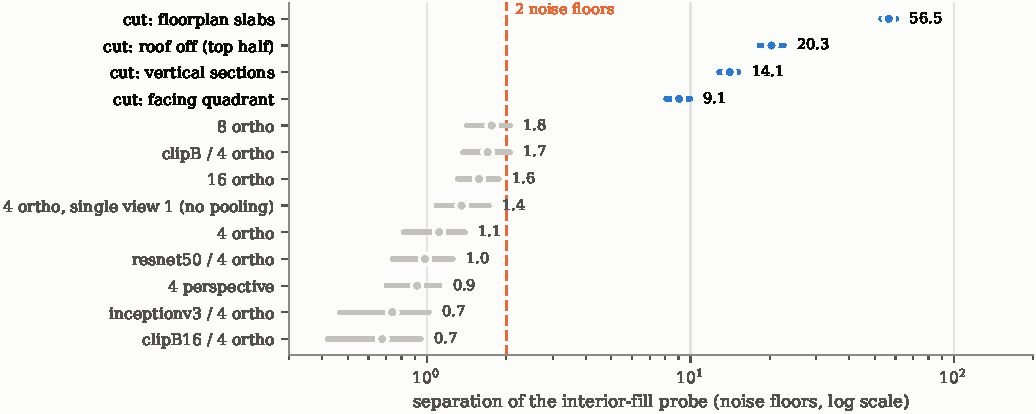
\includegraphics[width=0.9\linewidth]{figures/fig5_ablation}
\caption{\textbf{The blindness belongs to the view protocol, not the encoder.}
Separation of the interior-fill probe in each condition's own noise floors (log
scale), with paired bootstrap intervals. Gray: every encoder, view budget and
projection we test on exterior views, spanning $0.7$--$1.8$ floors. Blue: the
same encoder and the same statistic once the renders expose the interior.}
\label{fig:ablation}
\end{figure}

\begin{table}[!htb]
\centering
\small
\caption{The in-domain ladder at $n{=}128$, each statistic in its own noise floors,
measured from the floor's mean rather than from zero, so these values are not directly
comparable with Table~\ref{tab:ablation}'s. \textbf{All seven miss \solidify{} and resolve
every other corruption.}}
\label{tab:seven}
\begin{tabular}{lrrr}
\toprule
statistic & \solidify{} & $20\%$ deleted & \matshuffle{} \\
\midrule
KID & $\mathbf{2.0}$ & 12.3 & 132.3 \\
MMD-RBF & $\mathbf{2.1}$ & 13.9 & 148.8 \\
Fr\'echet distance & $\mathbf{0.5}$ & 10.8 & 72.4 \\
$1-$coverage & $\mathbf{0.2}$ & 7.7 & 19.8 \\
$1-$density & $\mathbf{0.1}$ & 7.2 & 14.0 \\
$1-$precision & $\mathbf{-0.4}$ & 9.0 & 28.0 \\
$1-$recall & $\mathbf{0.4}$ & 1.4 & 30.7 \\
\bottomrule
\end{tabular}
\end{table}

\begin{table}[!htb]
\centering
\footnotesize
\caption{Separation of \solidify{} from real in each condition's own noise floors
($n{=}256$, paired bootstrap, $95\%$ intervals). \textbf{Every exterior condition lands
between $0.7$ and $1.8$ noise floors; cutaways reach $9$--$57$ with the same encoder and
the same statistic.}}
\label{tab:ablation}
\begin{tabular}{llr@{\hspace{0.6em}}lc}
\toprule
& condition & \multicolumn{2}{c}{separation} & sees interior? \\
\midrule
\multirow{5}{*}{\rotatebox{90}{\footnotesize encoder}}
& DINOv2-B (ours) & $+1.1$ & {\footnotesize[0.8, 1.4]} & no \\
& CLIP ViT-B/16 & $+0.7$ & {\footnotesize[0.4, 0.9]} & no \\
& CLIP ViT-B/32 & $+1.7$ & {\footnotesize[1.4, 2.1]} & no \\
& ResNet-50 (ImageNet-supervised) & $+1.0$ & {\footnotesize[0.7, 1.3]} & no \\
& Inception-v3 pool3 (the FID backbone) & $+0.7$ & {\footnotesize[0.5, 1.0]} & no \\
\midrule
\multirow{3}{*}{\rotatebox{90}{\footnotesize views}}
& $8$ orthographic & $+1.8$ & {\footnotesize[1.4, 2.1]} & no \\
& $16$ orthographic & $+1.6$ & {\footnotesize[1.3, 1.9]} & no \\
& perspective & $+0.9$ & {\footnotesize[0.7, 1.1]} & no \\
\midrule
\multirow{3}{*}{\rotatebox{90}{\footnotesize \textbf{cut}}}
& \textbf{facing quadrant removed} & $\mathbf{+9.1}$ & {\footnotesize[8.1, 10.0]} & \textbf{yes} \\
& \textbf{roof removed} & $\mathbf{+20.3}$ & {\footnotesize[18.3, 22.6]} & \textbf{yes} \\
& \textbf{floorplan cross-sections} & $\mathbf{+56.5}$ & {\footnotesize[53.0, 60.5]} & \textbf{yes} \\
\midrule
& \vkid{} (no rendering at all) & $+120.8$ & {\footnotesize[115.7, 126.3]} & yes \\
\bottomrule
\end{tabular}
\end{table}

\section{What a Render Protocol Provably Cannot See}
\label{app:hull}

%TL;DR of paragraph: a deterministic renderer induces equivalence classes on which every render-and-embed metric is constant.
A deterministic render pipeline $R_V$ with a fixed view set $V$ induces an
equivalence relation on structures: $x \sim x'$ exactly when
$R_V(x) = R_V(x')$.

\begin{lemma}[Render kernel]\label{lem:kernel}
If $x \sim x'$ then $T(\mathcal{E}(R_V(x))) = T(\mathcal{E}(R_V(x')))$ for every
encoder $\mathcal{E}$, every pooling rule and every statistic $T$.
\end{lemma}
\begin{proof}
Immediate: the composition is a function of $R_V(x)$ alone.
\end{proof}

%TL;DR of paragraph: the lemma is only interesting because our own probe lands inside a class, which needs two more facts.
On its own Lemma~\ref{lem:kernel} is a tautology. It becomes a statement about
this paper because \solidify{} lands inside an equivalence class, which needs
two further facts.

\begin{lemma}[Surface invariance]\label{lem:surface}
\solidify{} leaves the exterior-air region unchanged, and leaves every exterior
face unchanged in cell, direction and material.
\end{lemma}

\begin{lemma}[Occlusion]\label{lem:occl}
Assume (a) nearest-surface shading, (b) faces bordering exterior air are opaque,
and (c) every camera lies outside the bounding box. Then
$R_V(\solidify(x)) = R_V(x)$ for \emph{every} view set $V$.
\end{lemma}
\begin{proof}[Proof sketch]
Any ray reaching a newly filled cell must first cross a face bordering exterior
air. By (b) that face is opaque and by (a) it is what the ray returns, so no
pixel can depend on the filled interior.
\end{proof}

%TL;DR of paragraph: the surface-invariance lemma also kills point-cloud and chamfer metrics, exactly.
Lemma~\ref{lem:surface} has a consequence beyond rendering. Any metric computed
on samples of the \emph{exterior surface} is a function of that face set, so it
too is constant under \solidify{}. We verify it: sampling exterior face centers
from a build and from its solidified copy gives \textbf{identical point sets on
$128$ of $128$ builds}, so chamfer distance, earth-mover distance and every
other point-cloud distance between them is exactly zero. This matters for the
proposal to replace renders with surface samples
\citep{luan2026rendermetric}, and for this corpus in particular: the model
released with it \citep{chen2019voxelcnn} reports a cumulative chamfer distance.
Sampling \emph{all} exposed faces, including those bordering sealed cavities,
does see the probe (mean chamfer $0.485$), but a surface sampler that reached
interior cavity walls would be observing the interior, which is the thing at
issue.

%TL;DR of paragraph: the conclusion, and the measurement that separates the exact regime from the leaky one.
Together with Lemma~\ref{lem:kernel} this is an impossibility result, not a
statistical one: under an opaque renderer \emph{no} encoder, statistic, sample
size or view budget separates a corpus from its solidified copy. We verify
Lemma~\ref{lem:surface} exhaustively ($0$ violations over the $399$ held-out
builds, and $0$ for \hollow{}) and Lemma~\ref{lem:occl} by rendering, using
counterfactual texture libraries to switch each hypothesis off in turn. The four
rows below are one experiment over the same $1{,}024$ (build, view) pairs, so
they are comparable to each other; the $91\%$ and $1.75\%$ quoted in
\S\ref{sec:hollow} come from a separate sweep of the whole test split
($399$ builds, $1{,}596$ views), which is why the deployed row here reads
$1.67\%$ rather than $1.75\%$. The two agree to within the difference between a
subsample and a census, and we keep each number with its own experiment rather
than mixing them:

\begin{center}\small
\begin{tabular}{lrrr}
\toprule
renderer & bit-identical & px changed (med.) & max ch.\ (med.) \\
\midrule
opaque, flat tiles (Lemma~\ref{lem:occl}) & $\mathbf{100.0\%}$ & --- & --- \\
flat tiles, translucency on & $62.5\%$ & $0.80\%$ & $94$ \\
textured, translucency off & $8.1\%$ & $0.99\%$ & $78$ \\
\textbf{deployed} (textured, translucency on) & $8.6\%$ & $1.67\%$ & $211$ \\
\bottomrule
\end{tabular}
\end{center}

%TL;DR of paragraph: our renderer violates hypothesis (b) twice, once physically and once as an artifact we disclose.
Our renderer violates hypothesis (b) in two ways, and the two have different
standing. The first is physical: Minecraft glass is translucent, so a
window in front of a filled void reveals the fill. This is a real channel, and
it is why the deployed figure is $91\%$ rather than $0\%$. The second is an
artifact of our mesh builder, which we report because it inflates that count.
\texttt{build\_mesh} assigns texture-atlas tiles in face-iteration order over
\emph{all} exposed faces, interior ones included; deleting interior faces
changes the tile count, hence the atlas layout, hence every UV rectangle, and
the sampler is nearest-neighbor. Switching translucency off still leaves $92\%$
of views altered by this alone, and within that condition ``atlas unchanged''
predicts bit-identity at $98.7\%$ agreement. A reader should therefore take
$91\%$ as a property of our renderer, not of the corruption; the corruption's
own reach is the $28\%$ that survives flattening the textures.

%TL;DR of paragraph: rescoring the probe through all four renderers shows the residual is wobble, not partial detection.
We then rescored the probe end to end through each of the four pipelines, holding
the arms, the draw and the estimator fixed and changing only the texture pack.
This turns the lemma into a prediction the benchmark either satisfies or does
not:

\begin{center}\small
\begin{tabular}{lrc}
\toprule
renderer & \mvkid{} separation & features identical \\
\midrule
opaque, flat tiles & $\mathbf{+0.000}$ & \textbf{yes} \\
flat tiles, translucency on & $-0.069$ & no \\
textured, translucency off & $+0.026$ & no \\
deployed & $+0.119$ & no \\
\bottomrule
\end{tabular}
\end{center}

The prediction holds exactly: bit-identical renders give bit-identical features
and therefore an identical kernel distance, so the separation is $0$ as an
identity rather than as a rounded measurement. The other three rows carry the
more useful lesson. The residual the benchmark reports for this probe is not a
small signal. It is \emph{wobble}. Changing only the texture pack, which
changes nothing whatever about the geometry being probed, moves it from $+0.26$
to $+0.03$ to $-0.16$: a range wider than the value itself, and one that crosses
zero, with the probe reading \emph{closer} to real than real does. This is what
it looks like when a metric is flat on an axis rather than weakly sensitive to
it, and it is why we argue the point by magnitude and ordering rather than by
the residual's sign. (The deployed row reads $+0.26$ here against the
leaderboard's $+0.38$ for the same quantity; the two runs estimate their own
floors, $0.00358$ and $0.00306$, which is the effect Appendix~\ref{app:nscale}
documents.)

%TL;DR of paragraph: where the surviving signal is lost, stated as measurement rather than theory.
Where the surviving signal dies is measurable but not, we think, provable. In
DINOv2 the patch tokens a changed pixel touches move by $0.062$ against a
between-build scale of $0.517$ ($12\%$); the CLS token moves $0.011$ against
$0.277$ ($3.9\%$); the four-view pooled embedding moves $0.0053$ against
$0.268$ ($2.0\%$). The signal enters the features and is attenuated by
aggregation. We report this as a measurement and decline the tempting story
that the encoder is invariant to the corruption by training, which the
patch-level numbers contradict.

%TL;DR of paragraph: the converse lemma, which makes the complementary-blindness claim symmetric.
The converse holds by the same style of argument and makes the paper's
complementarity claim provable on both sides rather than measured on one.

\begin{lemma}[Material blindness of \vkid{}]\label{lem:matblind}
The descriptor of \S\ref{sec:metrics} factors through the occupancy mask, so any
transformation preserving occupancy, \matshuffle{} and \monochrome{} among them,
leaves
it pointwise unchanged, and \vkid{} returns the real arm's value exactly.
\end{lemma}

Verified: descriptors are bit-identical (max difference $0.0$) and \vkid{}
returns the identical float for all three arms. The $+0.00$ printed in
Table~\ref{tab:leaderboard} is an identity, not a rounded measurement. Renders
of those same builds are never identical ($0$ of $256$ views; a median $25\%$ of
pixels move), so material permutation provably escapes the render kernel exactly
as interior fill provably falls inside it.

\section{Reading a Squared Statistic Over a Population of Prompts}
\label{app:failrate}

Everything in the main text concerns what a metric can \emph{see}. How its value is
\emph{read} is a second issue, and it affects any leaderboard reporting KID or MMD over a
population of prompts. Because these statistics are squared, an arm that fails on a quarter
of its builds scores only $6.4\%$ of the way to fully bad, where a reader assuming
proportionality would infer a quarter of the damage. Reporting the square root recovers the failure rate to a mean absolute error of $0.013$
against $0.128$ for the raw value.


A generator fails on a subset of prompts rather than uniformly. For a squared-MMD
statistic the response to such a mixture is quadratic,
\begin{equation}
\mathrm{MMD}^2\!\left(\alpha P + (1-\alpha)Q,\; P\right)
  = (1-\alpha)^2\,\mathrm{MMD}^2(Q, P),
\label{eq:mixture}
\end{equation}
a one-line consequence of the linearity of the mean embedding.
\citet{binkowski2018kid} state this identity in their Appendix B.2, and both they and
\citet{heusel2017fid} plot their metrics against a contamination fraction. We add the
reporting recommendation it implies: report $\mathrm{MMD} = \sqrt{\mathrm{MMD}^2}$, which
is \emph{linear} in the contaminated fraction and free to compute. The identity holds for
squared integral probability metrics such as KID and MMD. It does not hold for
Fr\'echet distance, which \citet{binkowski2018kid} show is not polynomial in $\alpha$,
so we derive the correction for KID only.


%TL;DR of paragraph: the measured exponent, the compression it causes, and what the square root recovers.
Measured on a mixture ladder whose bad pool is \randomvox{} at $n{=}128$, the best-fit
exponent is $\mathbf{1.99}$ against the identity's $2$. An arm failing on a quarter of
its builds scores $6.4\%$ of the way to fully bad ($0.110$ against $1.718$). Reporting
$\sqrt{\mathrm{KID}}/\sqrt{\mathrm{KID}_{\text{worst}}}$ recovers the true bad fraction
to a mean absolute error of $\mathbf{0.011}$ (\mvkid{}) and $\mathbf{0.022}$ (\vkid{}),
against $0.124$ and $0.135$ for the raw values.

%TL;DR of paragraph: the estimator is unbiased for the square, not its root, so the readout is a diagnostic rather than a ranked quantity.
One caution on the readout. The identity holds for the population quantity, while we
report an unbiased estimator of $\mathrm{MMD}^2$, which can be negative and whose square
root is therefore biased downward by Jensen's inequality, worst where the statistic is
small relative to its own standard error. We report the square root as a diagnostic for
reading a failure rate, never as the ranked quantity.

\section{What BlockScore's Maximum Is, Statistically}
\label{app:blockscore}

%TL;DR of paragraph: a max over k pillars has a positive null, so a fresh real arm scores about 1.1 rather than 0.
\blockscore{} is the maximum of five pillar scores, and a maximum of several
mean-zero quantities is not itself mean-zero. The control arm reads exactly
$0.00$ on every pillar because it \emph{is} the arm the calibration is taken
from: $(v_p - v_p)/\mathrm{sd}_p = 0$ identically, with zero variance. That is
an identity, not a measurement, and Table~\ref{tab:leaderboard} labels it as
such. A \emph{fresh} real arm, drawn from the same distribution but not used to
calibrate, scores $\mathbb{E}[\blockscore] = 1.08$ with standard deviation
$0.89$, right-skewed ($+0.89$), and a $95$th percentile of $2.8$. Read
\blockscore{} against that null rather than against zero: a value of $15$ is not
``$15$ standard deviations'' but ``far outside a null whose upper tail is under
$3$''. The inflation is about one noise floor, against a smallest ranked score
of $60.8$, so it changes no ordering and no conclusion in this paper. A
future suite comparing arms that sit within a few floors of real would need to
subtract it.

%TL;DR of paragraph: three pillars are in real noise floors and two are in a coarser unit, so the max is a veto over three.
The five pillars are not in one unit. Appearance, geometry and palette are
divided by a genuine sampling noise floor, and we verify this: their declared
units match the spread of fresh real draws to within $7\%$ ($0.93$, $1.03$ and
$1.05$ of the measured value). The coherence and geometry-scalar pillars are
divided by a per-build robust spread of the reference, an effect size measuring how
far apart two distributions are in units of how much individual builds differ
Measurement puts that unit $29\times$ and $52\times$ coarser than those
pillars' own sampling noise. A structure pillar would therefore have to move
some $1{,}800$ of its actual noise floors to veto a live pillar sitting at
$+60$, and on our card none ever does. We state this as a limitation of the
current calibration rather than a property of the aggregation rule: the maximum
is the right rule, and two of the five inputs are quoted in a unit that makes
them diagnostics rather than vetoes.

%TL;DR of paragraph: the number is only interpretable beside the name of the pillar that produced it.
One consequence for reporting. Because the winning pillar's unit is what the
number is in, \blockscore{} is uninterpretable without the pillar that produced
it, which is why every leaderboard we print carries a \emph{worst pillar}
column. It is also not convertible to a $p$-value: the null is max-shaped and
skewed, so the usual normal reading does not apply.

\section{The Noise-Floor Unit Depends on $n$}
\label{app:nscale}

Separations throughout this paper are quoted in \emph{noise floors}: the
standard deviation of repeated real-versus-reference draws at the same sample
size. That unit makes two metrics with incommensurable raw scales comparable
within a run, which is why we use it. It is not scale-free across runs,
and we state the dependence explicitly because it is easy to misread.

Measured on the identical corruption at two sample sizes:

\begin{center}
\small
\begin{tabular}{lrrrrrr}
\toprule
metric & sd $n{=}64$ & sd $n{=}128$ & ratio & sep $n{=}64$ & sep $n{=}128$ & ratio \\
\midrule
\vkid{} & 0.1732 & 0.0848 & \textbf{0.49} & 132.9 & 286.7 & \textbf{2.16} \\
\mvkid{} & 0.00449 & 0.00331 & 0.74 & 0.4 & 1.1 & 2.84 \\
\bottomrule
\end{tabular}
\end{center}

The noise floor of the geometric metric halves when $n$ doubles, the $1/n$ decay
expected of a degenerate U-statistic under the null, while the
population effect is fixed. A separation in noise floors therefore grows
\emph{linearly} in $n$, and a figure such as ``$202$'' means ``$202$ at
$n{=}128$''; the same measurement at $n{=}256$ reads roughly $400$.

Three practical consequences. Separations are only comparable across runs at
equal $n$, which is why our protocol pins it. Cross-domain figures must be
normalized before they are set side by side. And regenerating every arm at a
larger $n$ leaves the \emph{ordering} of arms intact while roughly doubling
every magnitude, and the orderings are what our conclusions rest on.

\paragraph{The unit is estimated, not only $n$-dependent, and equal $n$ is not
enough.} The floor is itself a statistic: $48$ real-versus-reference draws,
carrying a relative standard error near $1/\sqrt{2 \cdot 47} \approx 10\%$.
Two of our own runs make the consequence concrete. At the same $n{=}128$, the
same corpus, the same pinned split, the same reference and the same commit, the
leaderboard run of record reports the interior-fill separation as
$\mathbf{201.8}$ and the converse-probe run reports it as $\mathbf{286.7}$.
The only differing inputs are two random seeds, one choosing which $128$ test
builds were drawn and one seeding the $48$ floor draws. The ratio decomposes
exactly into the two:
\[
\underbrace{\frac{286.7}{201.8}}_{1.42}
\;=\;
\underbrace{\frac{0.1097}{0.0848}}_{\text{floor estimate, } 1.29}
\;\times\;
\underbrace{\frac{24.430 - 0.128}{22.034 - (-0.095)}}_{\text{raw difference, } 1.10},
\]
that is, roughly $70\%$ a different estimate of the same floor and $30\%$ a
different draw of the builds. Two estimates of one floor landing $29\%$ apart is
a $2\sigma$ event for a standard deviation taken from $48$ draws, so the unit
carries a visible error bar. A separation should therefore be read to one or two
significant figures, with its run named. We quote $202$ throughout because it is
the run of record's value, and the reader should understand it as \emph{about two
hundred}: a sweep over twelve seeds places it between $185$ and $274$.

\paragraph{The linear-in-$n$ rule holds at fixed reference size.} The
prediction above, that $n{=}256$ reads roughly $400$, assumes the reference
pool is unchanged. Our view-protocol ablation measures the same probe on the
same corpus and split at $n{=}256$ and reads $120.8$, not $400$, because it
scores against $512$ reference builds rather than $399$ and its floor
($0.188$) is consequently \emph{larger} than the $n{=}128$ floor rather than
half of it. The rule describes how a separation moves when $n$ grows within one
protocol; it does not survive a change of reference. This is the same caution as
the cross-domain one, and it is why every number in this paper is reported with
its run.

\paragraph{A note on what the ladder tables difference against.} The
per-metric ladder artifacts (Table~\ref{tab:ladder-render}) express a rung as
its distance from the null \emph{mean}, while the leaderboard expresses an arm
as its distance from a held-out \realheld{} \emph{draw}. On an exactly
invariant rung the two conventions differ by construction: the geometry metric's
material-shuffle row is $0$ exactly against the \realheld{} draw and $1.19$
against the null mean. The conventions must not be mixed within one comparison.

\mvkid{} scales less cleanly ($0.74$ rather than $0.49$) because its separation
is a ratio of two quantities that are both near zero. That is the finding rather
than a defect of the unit: the render row should be read as
``indistinguishable'', not as a number.

\section{Calibration of the Head-to-Head Test}
\label{app:significance}

%TL;DR of paragraph: the paired test we first used was anti-conservative, we replaced it with a permutation test, and we report what changed.
Our first implementation estimated the standard error of a paired difference by
subsampling $80\%$ of each arm without replacement and using the spread of those
draws directly. That is the variability of a subsample statistic around the
full-sample value, which becomes the standard error of the full-sample statistic
only after a rescale we did not apply. Measured on exact nulls, the resulting
test rejected $3.4\times$ too often at $\alpha{=}0.05$ when the arms match the
reference and $7.2\times$ too often when they do not.

%TL;DR of paragraph: no single rescale works because the statistic changes regime, so we use a permutation test.
No constant rescale repairs it. Conditional on a fixed reference, the difference
of kernel distances is a degenerate U-statistic when both arms match the
reference and a non-degenerate one when they do not, with required factors of
$1.31$ and $2.06$ respectively; across the $153$ pairs of one table the factor
ranges from $0.30$ to $11.9$. We therefore use an exact label-permutation test:
pool the two arms, re-split at the observed sizes, and recompute the difference
against the same fixed reference. Its null standard deviation tracks a
Monte-Carlo ground truth within $5\%$ in both regimes, and its type-I error is
nominal at both levels.

%TL;DR of paragraph: recomputing the run of record leaves both null results intact and costs two positive separations.
Recomputing the run of record changes only claims of separation, which is the
expected direction: a test that rejects too easily can manufacture a difference
but never a tie. Both of our null results hold and strengthen: \solidify{}
remains unseparated from held-out real ($p$ from $0.61$ to $0.77$), and the clean
retrain remains unseparated from the language-model baseline ($0.89$ to $0.93$).
Two positive separations do not survive: \traincopy{} against held-out real falls
to the $\alpha{=}0.05$ boundary, and the contaminated arm separates from one
language-model baseline but not the other. We report the blindness result by
magnitude for this reason, and the case study's conclusion, that the contaminated
arm's apparent advantage does not survive a clean split, is
unaffected, since it rests on a within-architecture comparison.

\section{Additional Figures}
\label{app:figures}

\begin{figure}[!htb]
\centering
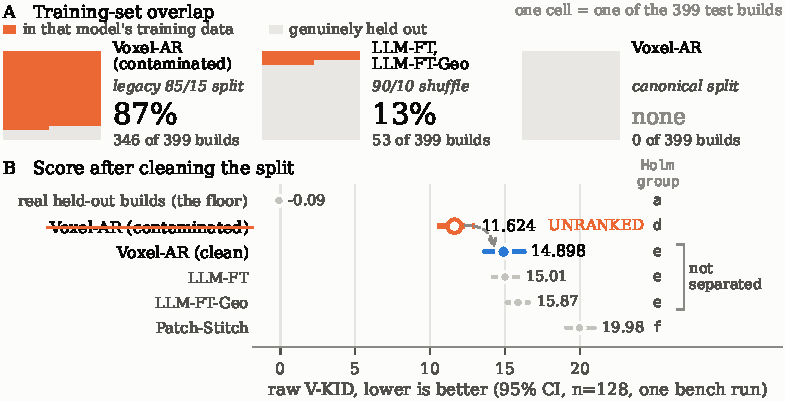
\includegraphics[width=0.90\linewidth]{figures/fig_contamination}
\caption{\textbf{Declared provenance, and what it cost.} \emph{A:} how much of the
canonical test split each arm had already trained on; the third waffle is \voxar{}
retrained on that split. \emph{B:} the retrain costs $+3.27$ raw \vkid{} and erases the
margin. No memorization gate fires on the contaminated arm, so it is unranked rather than
disqualified.}
\label{fig:contamination}
\end{figure}

\begin{figure}[!htb]
\centering
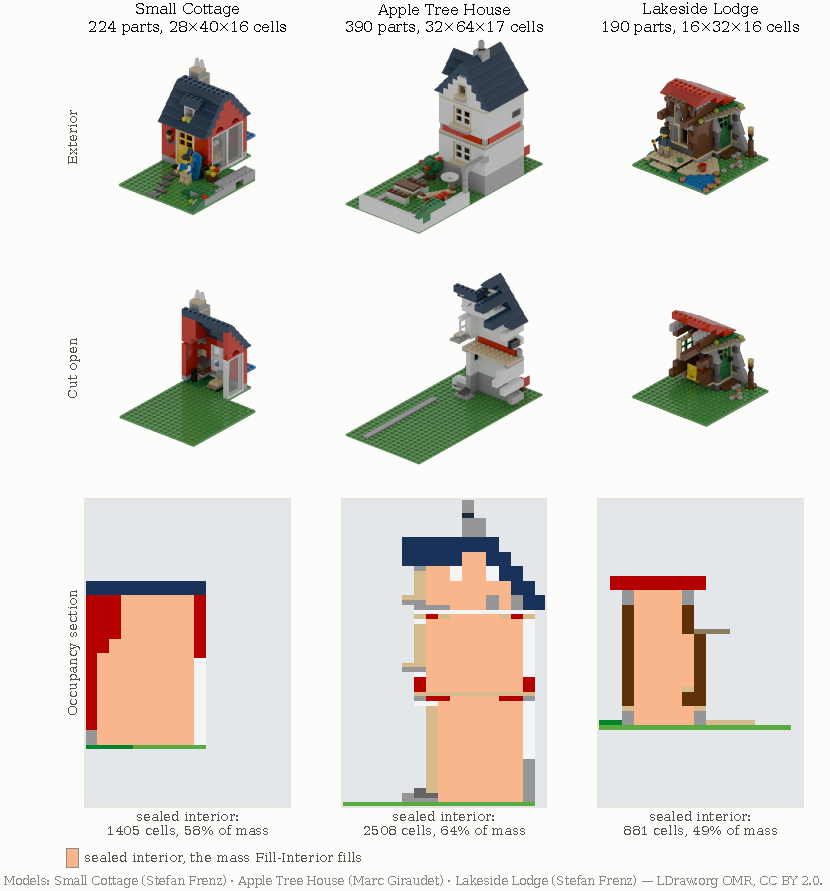
\includegraphics[width=0.72\linewidth]{figures/fig8_lego_omr}
\caption{\textbf{A second domain, with real colors.} Three LDraw.org OMR models in their
own LEGO colors: the exterior an exterior protocol sees, the same parts cut past one
plane, and the occupancy grid we derive sliced at that plane, sealed interior in peach,
every other color the parts' own, all renders at one scale. This domain shares only the
fact that builds enclose space: different parts, different lattice, different renderer, $190$--$390$ parts against
thousands of blocks. The measured replication of
\S\ref{sec:lego} runs on StableText2Brick rather than on these three models, which we
picture because their terms permit it (Appendix~\ref{app:data}). Official LEGO sets are
far less hollow than either measured corpus: among models with at least eight sealed cells,
the basis the OMR audit reports, \solidify{} adds a median $+1.2\%$ mass to an OMR model
against $+35.8\%$ to a held-out house. Models: Small Cottage (Stefan Frenz), Apple Tree House (Marc Giraudet), Lakeside
Lodge (Stefan Frenz); LDraw.org OMR, CC BY 2.0, modified only by the deletions shown.}
\label{fig:lego}
\end{figure}

\begin{figure}[!htb]
\centering
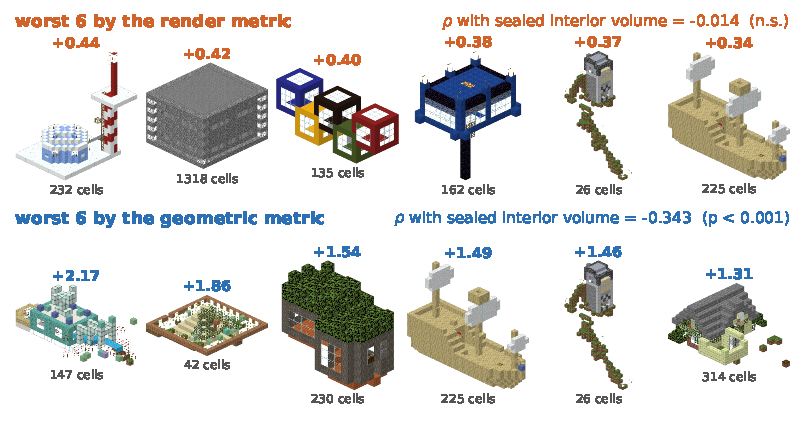
\includegraphics[width=\linewidth]{figures/fig11_influence}
\caption{\textbf{The two metrics disagree about real builds, with no probe involved.} The
unbiased estimator is a sum over builds, so each build's contribution to its arm's score is
recoverable. The six builds each metric penalizes most are shown with their contribution and
their sealed interior volume. The two orderings are nearly independent, $\rho = +0.167$, and
only the geometric ordering tracks how much interior a build has: its rank correlation with
sealed interior volume is $-0.343$ ($p < 0.001$) against $-0.014$ for the render metric.
Builds shown are 3D-Craft only, for licensing.}
\label{fig:influence}
\end{figure}

\begin{figure}[!htb]
\centering
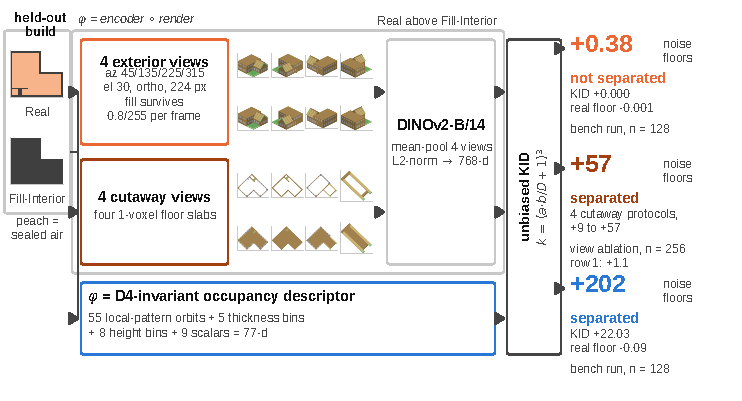
\includegraphics[width=0.95\linewidth]{figures/fig_pipeline}
\caption{\textbf{One estimator, three feature maps.} \mvkid{} and \vkid{} are the
same unbiased kernel distance of Eq.~\ref{eq:mmd} and differ only in $\phi$.
\emph{Row 1:} the render-and-embed path, where the structure reaches the statistic
as four images. \emph{Row 2:} the same renderer and the same encoder with cutaway
views, which recovers the signal. One renderer, one encoder, only the views
differ, and four other encoders and $8$ or $16$ views change nothing
(Table~\ref{tab:ablation}). \emph{Row 3:} the geometric path, which reads
occupancy directly and needs no renderer and no GPU. A noise floor is a run's own
real-vs-real spread and falls with $n$, so separations compare within a run: rows
$1$ and $3$ come from one scorecard at $n{=}128$ against $399$ reference builds,
and row $2$ from the view ablation at $n{=}256$, where row $1$ scores $+1.1$. The
sections at left are horizontal slices of one 3D-Craft build.}
\label{fig:pipeline}
\end{figure}

\begin{figure}[!htb]
\centering
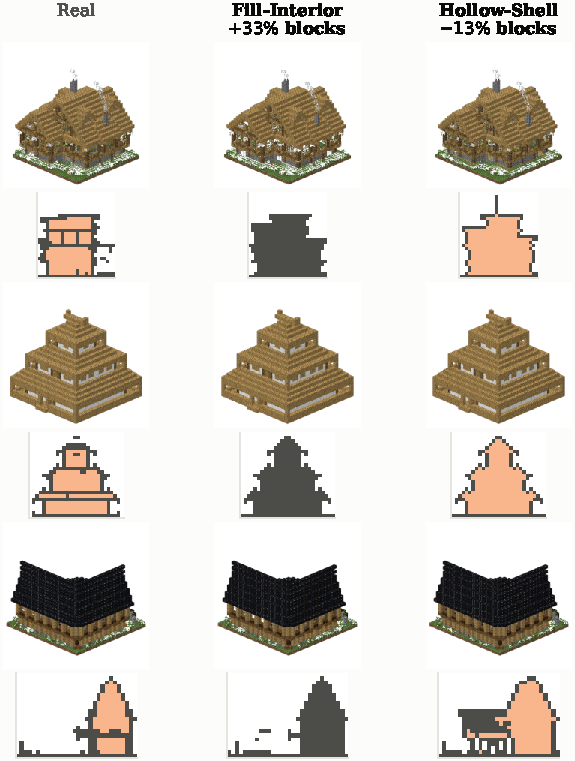
\includegraphics[width=0.60\linewidth]{figures/fig7_probe_gallery}
\caption{\textbf{Both directions of the corruption, on three held-out builds.}
\solidify{} adds a median $33\%$ blocks and \hollow{} removes a median $13\%$,
yet the views the metric is given are near-identical in every column. The
cross-sections show what changed, with sealed interior air in peach. \mvkid{} places both within one noise floor of
real ($+1.0$ and $+0.4$); \vkid{} places them $287$ and $156$ away.}
\label{fig:gallery}
\end{figure}

\begin{figure}[!htb]
\centering
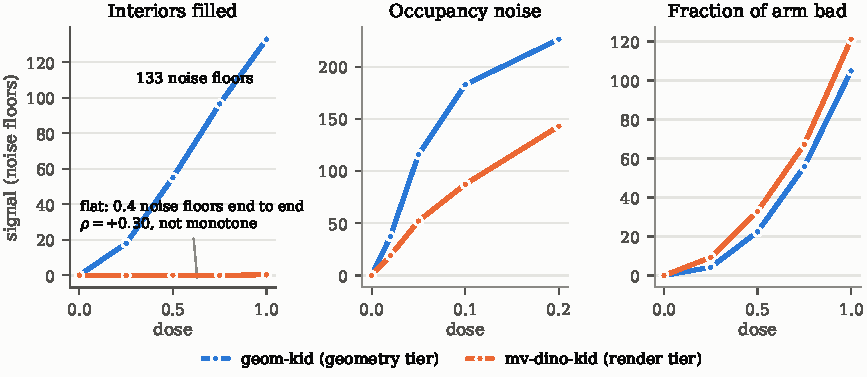
\includegraphics[width=0.95\linewidth]{figures/fig2_dose_response}
\caption{\textbf{Dose--response.} Each metric in units of its own noise floor,
which is the only scale on which the two are commensurable. Both rise
monotonically on occupancy noise and on the mixture axis; on the interior axis
the render metric does not move.}
\label{fig:dose}
\end{figure}

\begin{figure}[!htb]
\centering
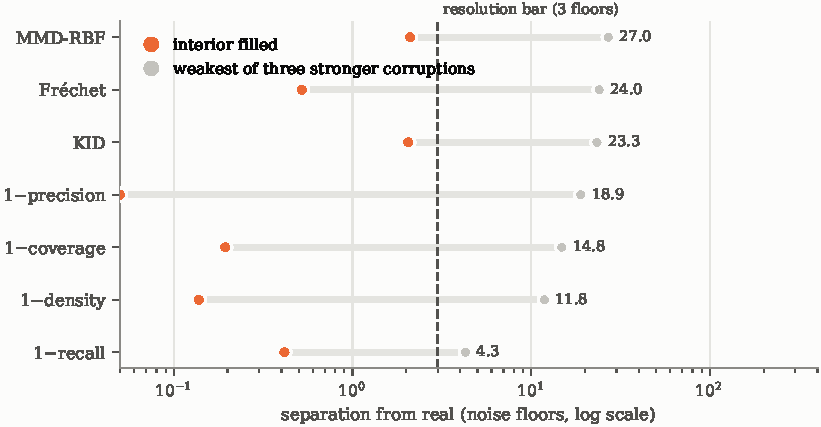
\includegraphics[width=0.86\linewidth]{figures/fig6_seven_statistics}
\caption{\textbf{Every render-space statistic shares the blindness} (LEGO,
$n{=}128$). Filled marker: the interior-fill probe. Open marker: the weakest of
three stronger corruptions. All seven resolve the stronger corruptions and none
resolves the interior fill. One minus recall also misses the milder
$20\%$-deletion rung at $1.4$ floors, a limit of that statistic rather than of
the probe.}
\label{fig:seven}
\end{figure}

\begin{figure}[!htb]
\centering
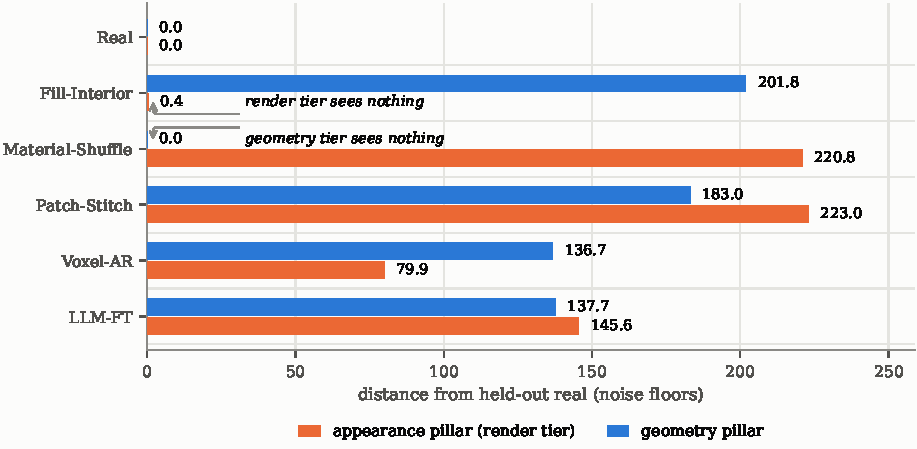
\includegraphics[width=0.88\linewidth]{figures/fig3_pillars}
\caption{\textbf{The two blindnesses are mirror images.} Distance from held-out
real on the two pillars. \solidify{} is invisible to the render tier and far from
real on geometry; \matshuffle{} is the exact converse, at precisely zero on
geometry.}
\label{fig:pillars}
\end{figure}

\begin{figure}[!htb]
\centering
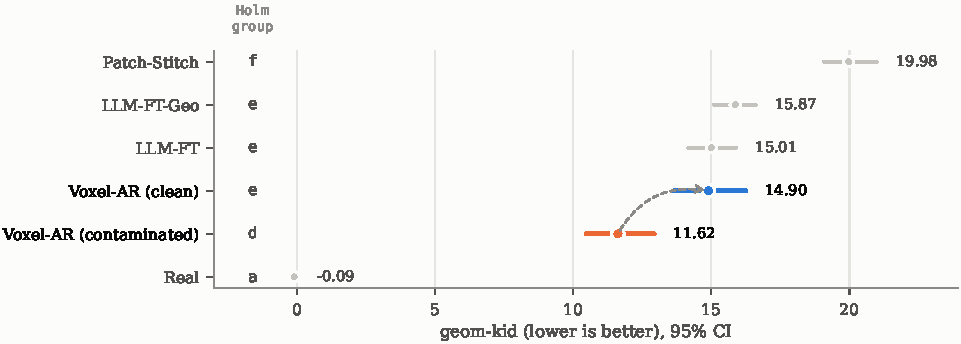
\includegraphics[width=0.9\linewidth]{figures/fig4_casestudy}
\caption{\textbf{The contamination case study.} \vkid{} with bootstrap intervals.
Cleaning the split moves \voxar{} out of group (d) and into a tie with the
baselines in group (e). The letters shown are from the original run; see
Appendix~\ref{app:significance} for the corrected compact letter display, under
which the contaminated arm does not hold a group alone.}
\label{fig:casestudy}
\end{figure}

\section{Data Provenance and Release}
\label{app:data}

%TL;DR of paragraph: what we release, what we do not, and why the corpus is reproducible without redistributing it.
Our Minecraft corpus derives from four public sources: the 3D-Craft house
dataset \citep{chen2019voxelcnn,gray2019craftassist}, released with the
CraftAssist project; a scrape of \texttt{grabcraft.com}; and the
text2mc dump, whose builds originate from \texttt{planetminecraft.com}. \textbf{We
do not redistribute the GrabCraft- or text2mc-derived structures.} GrabCraft's
terms permit sharing blueprints only by linking, and PlanetMinecraft's terms
prohibit redistributing site data. We release instead the curation code, the
per-build source URLs, content hashes, the group-aware split as index lists, and
a rebuild script, so the corpus reproduces bit-exactly without our distributing
third-party content. The four things the paper promises, namely the suite, the
probes, the baselines and the split, contain no upstream content.

%TL;DR of paragraph: published images are restricted by source, and the texture assets they use are permitted for non-commercial images but not redistributed.
Every build shown in this paper, and every stimulus shown to a human rater,
comes from \textbf{3D-Craft only}. GrabCraft's terms name pictures of blueprints
as a prohibited form of distribution; 3D-Craft's builds were commissioned as a
research corpus and carry no prohibition on depiction. Their license needs
stating precisely, because it is not the one the CraftAssist code carries. The
CraftAssist codebase is MIT, but the house data ships as a tarball with no
license file, and the release that distributes it for the 3D-Craft paper,
\texttt{facebookresearch/voxelcnn}, is CC BY-NC 4.0. We therefore treat the
corpus as non-commercial research material requiring attribution, which is what
our use and this paper's figures are, and we state that restriction on the
release rather than inheriting the code's MIT terms. Figures render these builds
with Minecraft's own texture assets, which are Mojang's copyright. Mojang's
usage guidelines permit non-commercial use of images of the game, and this
paper is non-commercial research; we also reproduce the attribution they
require, and nothing here suggests official endorsement. Two limits follow and
we observe both. The released code and data contain \textbf{no texture files},
so a reader reproducing our figures supplies them from their own installation.
And the permission covers the images, not the assets: we publish renders, never
the pack. The alternative would be flat per-block colors, which need no
permission at all because they leave only third-party-authored geometry, and
the figure scripts still produce them on request; we render with textures
because they show what the metric is actually given. Minecraft features: \copyright{} Mojang Synergies
AB, included courtesy of Mojang AB. This is not an official Minecraft product and
is not approved by or associated with Mojang or Microsoft.

%TL;DR of paragraph: attribution is by URL because creator names were never captured, and we say so.
Builds are credited by source URL in the released manifests. The original scrape
did not capture uploader names, so we cannot credit individual creators, and we
record that as a limitation rather than an omission. Our LEGO evaluation corpus
is StableText2Brick \citep{pun2025brickgpt}, loaded from HuggingFace and not
redistributed; it derives from ShapeNetCore, whose terms restrict use to
non-commercial research.
\TODO{Insert the institutional determination for the corpus release and the
human-subjects review before submission. Both are open questions for the
university's research-compliance office, not settled by the authors.}

\begin{figure}[t]
\centering
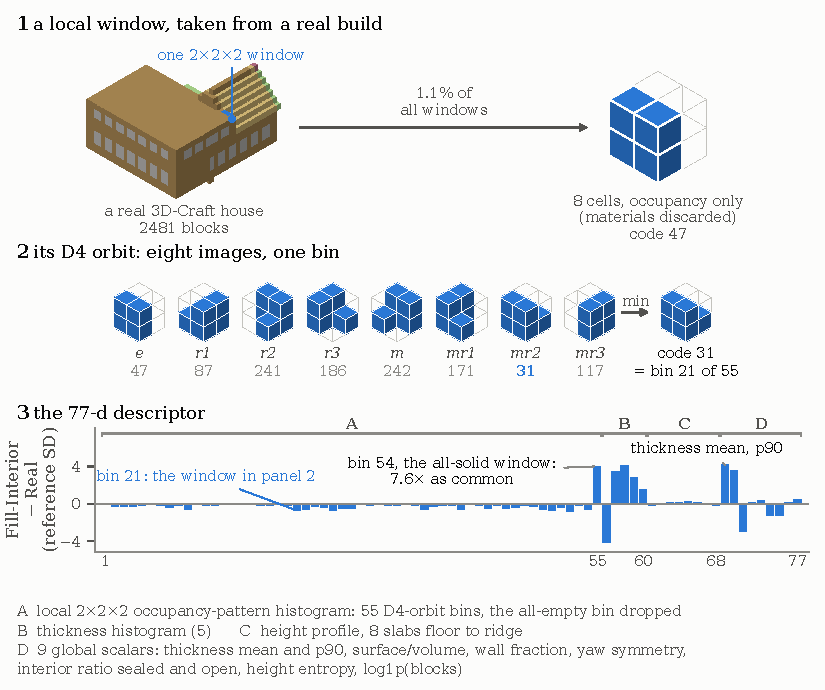
\includegraphics[width=0.92\linewidth]{figures/fig_descriptor}
\caption{\textbf{The geometric descriptor.} A $2\times2\times2$ occupancy
neighborhood, its orbit under the order-$8$ group of yaw rotations and an
$x$-mirror collapsing to one canonical bin, and the resulting feature vector with
the shift \solidify{} induces. The thickness histogram loses its one-block walls
and gains thick cores, and surface-to-volume with both interior ratios falls.
Filling every sealed interior moves this descriptor $202$ noise floors at
$n{=}128$, where the same builds move the render tier $0.4$.}
\label{fig:descriptor}
\end{figure}

\begin{figure}[p]
\centering
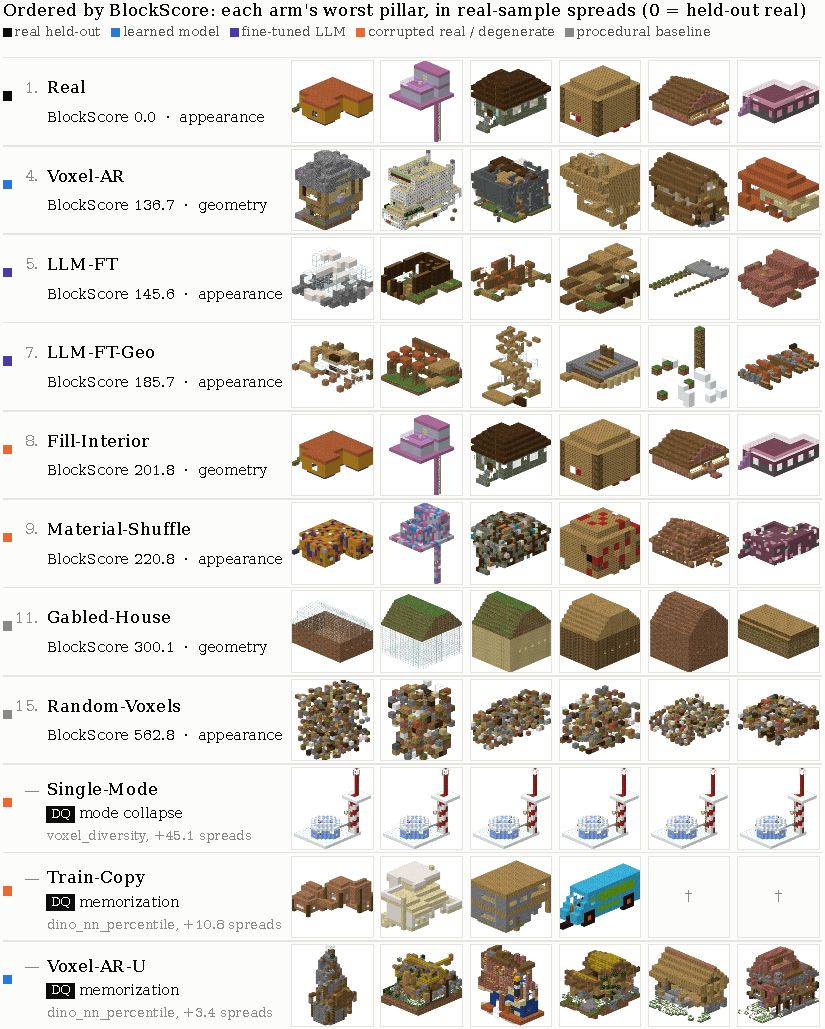
\includegraphics[width=\linewidth]{figures/fig_samples}
\caption{\textbf{Every arm, ordered by \blockscore{}.} Six builds per arm: the
first six the run recorded, in the seeded order it recorded them, topped up from
that arm's full scored sample where fewer than six remain. Builds one voxel
thick are passed over, since they draw as a hairline; a fifth of what the two
language-model arms emit is that shape, a truncation failure
\S\ref{sec:setting} describes. \realheld{}, \solidify{} and \matshuffle{} are
the same six buildings column for column, so a corruption reads down a column
and the paper's central claim can be checked by eye: the \solidify{} row scores
$+201.80$ and does not change. Each build is framed to its own bounding box, so cells are not to a common scale, and
\texttt{DQ} marks an arm a disqualification gate refused a rank
(Table~\ref{tab:leaderboard}). Cells marked $\dagger$ are withheld under
GrabCraft's terms; no build shown is a memorized copy, the nearest of $1{,}863$
training builds reaching IoU $0.51$. The contaminated checkpoint of
\S\ref{sec:casestudy} is absent: it is unrankable, and a gallery ordered by
score would imply a standing it does not have.}
\label{fig:samples}
\end{figure}
